\chapter{Distribuci\'on de Presi\'on en el Prot\'on}\label{ch:TotalPandGluons}

\fancyhf{} % clear all header fields
\fancyhead[LE]{\nouppercase{\textbf{Cap\'itulo 4. Distribuci\'on de Presi\'on en \\el Prot\'on}\hfill\textit{\rightmark}}}
\fancyhead[RO]{\nouppercase{\textit{\rightmark}\hfill\textbf{Cap\'itulo 4. Distribuci\'on de Presi\'on en \\el Prot\'on}}}
\fancyfoot[LE]{\nouppercase{\thepage\hfill {Distribución de la presión dentro de los nucleones en un modelo de bolsa de Tsallis-MIT}}}
\fancyfoot[RO]{\nouppercase{{Distribución de la presión dentro de los nucleones en un modelo de bolsa de Tsallis-MIT} \hfill \thepage}}

\begin{chaptersummary}
Este cap\'itulo desarrolla la extracci\'on de las distribuciones radiales de presi\'on dentro del prot\'on, combinando resultados de factores de forma gravitacionales (GFFs) con predicciones del modelo estad\'istico Tsallis-MIT. Se reconstruye la presi\'on de quarks $P_Q(r)$ a partir de datos fenomenol\'ogicos, se modela la presi\'on total $P_q(r)$ en un plasma no extensivo, y finalmente se extrae la contribuci\'on glu\'onica $P_G(r)$ por diferencia.
\end{chaptersummary}

\section{Presi\'on de Quarks desde Factores de Forma Gravitacionales}
La presi\'on interna de quarks $P_Q(r)$ se reconstruye a partir del t\'ermino $D$ de los factores de forma gravitacionales (GFFs), siguiendo:

\begin{equation}
d_1(t) = d_1(0) \left( 1 - \frac{t}{M^2} \right)^{-\alpha}
\end{equation}

con $d_1(0) = -2.04$, $M = 5\,\mathrm{fm}^{-1}$ y $\alpha = 3$.

La relaci\'on entre $d_1(t)$ y la distribuci\'on de presi\'on radial es:

\begin{equation}
P_Q(r) = -\frac{1}{k_p \pi^2} \int_0^\infty x^4 j_0(r x) d_1(-x^2) \, dx
\end{equation}

donde $j_0$ es la funci\'on de Bessel esf\'erica de primer tipo, y $k_p = 55$.

La soluci\'on anal\'itica es:

\begin{equation}
P_Q(r) = \frac{M^6 d_1(0)}{16\pi k_p r} e^{-M r}(M r - 3)
\end{equation}

Esta presi\'on quark es consistente con resultados experimentales recientes~\cite{Burkert_2018}.

\section{Presi\'on Total en el Modelo Tsallis-MIT}
La presi\'on total en el modelo estad\'istico Tsallis-MIT se calcula como:

\begin{equation}
P_q(r) = \frac{37\pi^2}{90} T(r)^4 + \frac{256\pi^2}{15}(1-q) V T(r)^7
\end{equation}

donde:
\begin{itemize}
\item $T(r) = T_0 e^{-r^2/R_T^2}$ es el perfil de temperatura radial,
\item $V = \frac{4}{3}\pi R_{bag}^3$ es el volumen fijo de la bolsa (\( R_{bag} \approx 0.8\,\mathrm{fm} \)).
\end{itemize}

Se asume que fuera de la bolsa la presi\'on glu\'onica se anula debido a la estructura de frontera.

\section{Extracci\'on de la Presi\'on Glu\'onica}
La contribuci\'on de gluones a la presi\'on se obtiene como la diferencia:

\begin{equation}
P_G(r) = P_q(r) - P_Q(r)
\end{equation}

\begin{figure}[h]
    \centering
    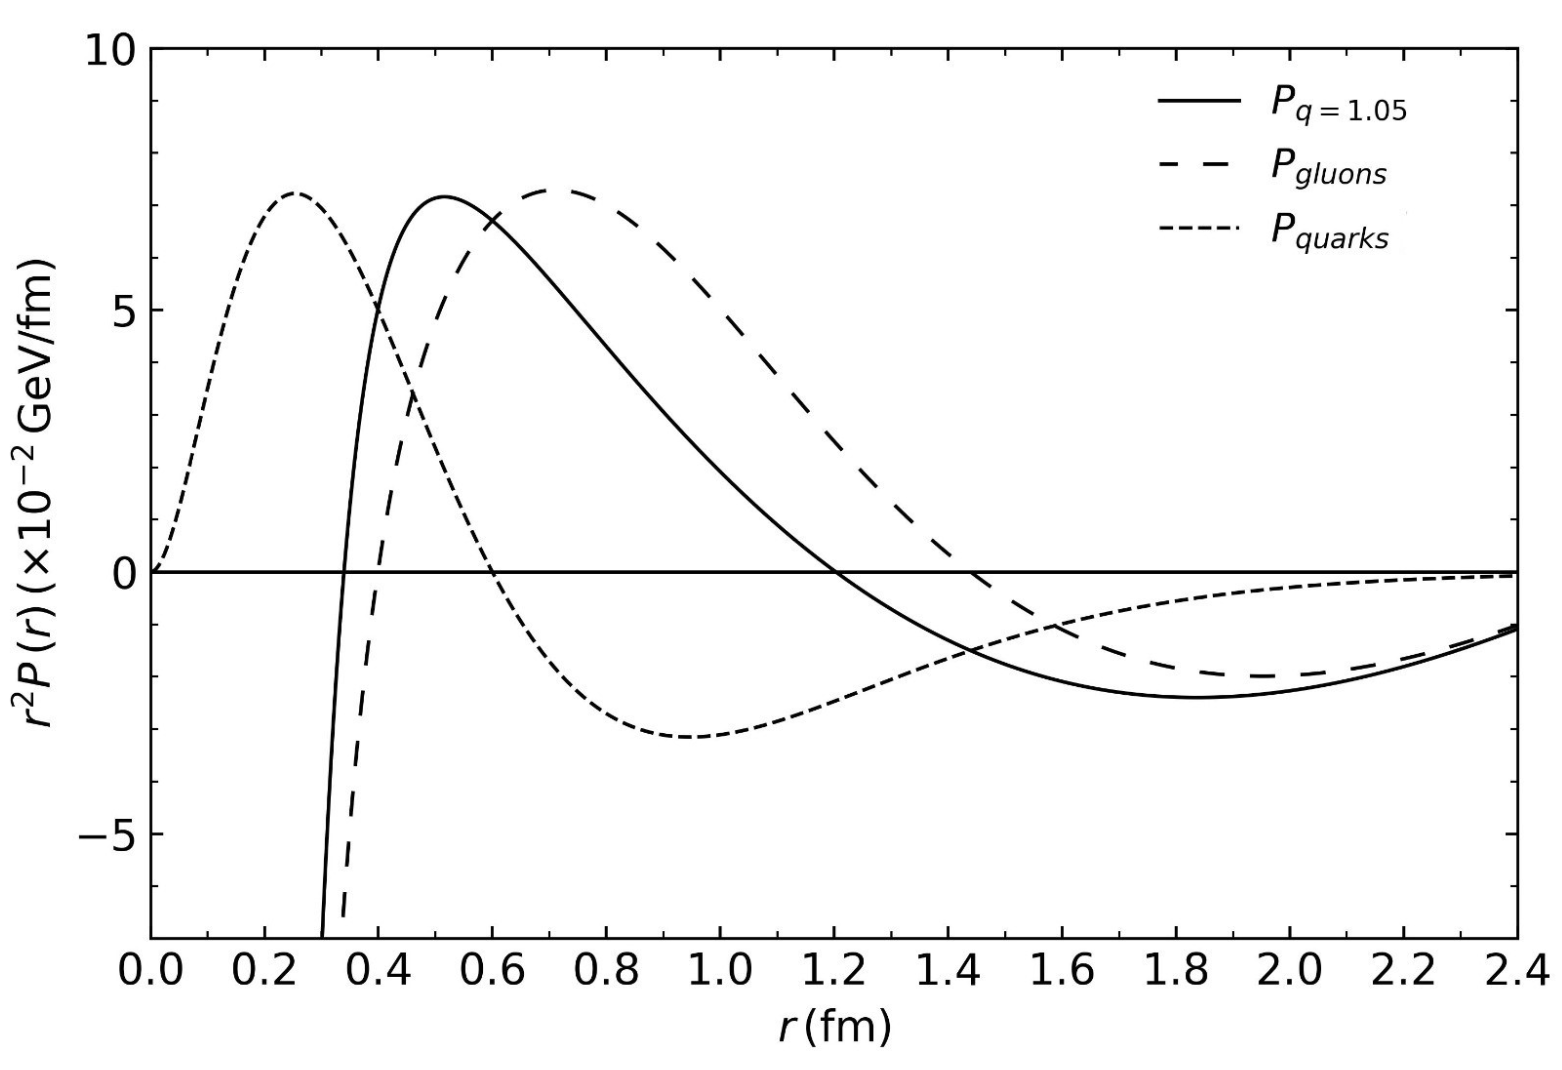
\includegraphics[width=0.8\textwidth]{./Images/PressureDistributionsTot-Q-G.png}
    \caption[Distribuciones radiales de presi\'on en el prot\'on]{Distribuciones radiales de presi\'on en el prot\'on: presi\'on total $P_q(r)$ (l\'inea continua), presi\'on glu\'onica $P_G(r)$ (l\'inea discontinua larga) y presi\'on de quarks $P_Q(r)$ (l\'inea discontinua corta) reconstruida de datos experimentales~\cite{Burkert_2018}.}
    \label{fig:PressureDecomp}
\end{figure}

\break

\section{Resultados Clave}

\begin{table}[h]
    \centering
    \caption{Propiedades de las distribuciones de presi\'on}
    \begin{tabular}{lccc}
    \toprule
    Componente & M\'aximo [GeV/fm$^3$] & Posici\'on del M\'aximo [fm] & Integral Total [GeV] \\
    \midrule
    $P_Q$ (quarks) & 0.35 & 0.3 & 1.04 \\
    $P_G$ (gluones) & -0.15 & 0.8 & -1.04 \\
    \bottomrule
    \end{tabular}
    \label{tab:PressureResults}
\end{table}

\section{Validaci\'on de la Condici\'on de Estabilidad}
Se verifica la condici\'on de estabilidad mec\'anica:

\begin{equation}
\int_0^\infty [P_Q(r) + P_G(r)] r^2 \, dr = 0
\end{equation}

lo cual garantiza el equilibrio interno del prot\'on. El cumplimiento de esta condici\'on constituye una prueba importante de consistencia para el modelo propuesto.

\begin{remark}[Detalles matemáticos]
    La deducci\'on completa de la expresi\'on de \( P_Q(r) \) a partir del t\'ermino \( d_1(t) \), as\'i como las consideraciones sobre unidades y constantes f\'isicas, se encuentran en el Ap\'endice~\ref{app:math_derivations}.
\end{remark}


% La distribución de presión total está dada por 

% \begin{equation}
% {P}_{q} =\left[\frac{7}{4}{g}_{Q} + {g}_{G} \right] \frac{{\pi}^{2}}{90}{T}^{4} + \frac{1}{12} {g}_{Q} \left[\frac{\mu}{T} \right]^{2} {T}^{4} + \frac{8{\pi}^{2}}{90} {g}_{Q}{g}_{G} \left(1-q\right) \left[\frac{{\pi}^{2}}{90} + \frac{1}{30} \left(\frac{\mu}{T} \right)^{2} \right]V{T}^{7} + C \left(V,\mu,q \right)
% \end{equation}

% con $C(V,\mu,q) = \frac{1}{2{\pi}^{2}}{\mu}^{4}$, donde para $q=1$ se recupera la presión total convencional de \gls{bg} es debido a los quarks y gluones y puede ser visto en la figura \ref{fig: Presión total en T-MIT bag model}. La presión está dada como una función del radio para varios potenciales químicos a parámetro $q$ fijo. Si se incrementa la densidad de las partículas a una temperatura dada, los hadrones eventualmente se ``romperán'', es decir, resultará en deconfinamiento. Esto pasa a densidades de aproximadamente $\nicefrac{0.72}{\mathrm{\unit{\femto\meter}}^{3}}$ o potenciales químicos por sobre el orden de $430 \mathrm{MeV}$[Referencia 35]. A altar temperaturas, la transición de fase sería alcanzable en densidades más bajas

% \begin{wrapfigure}{l}{0.58\textwidth}
% \centering
% 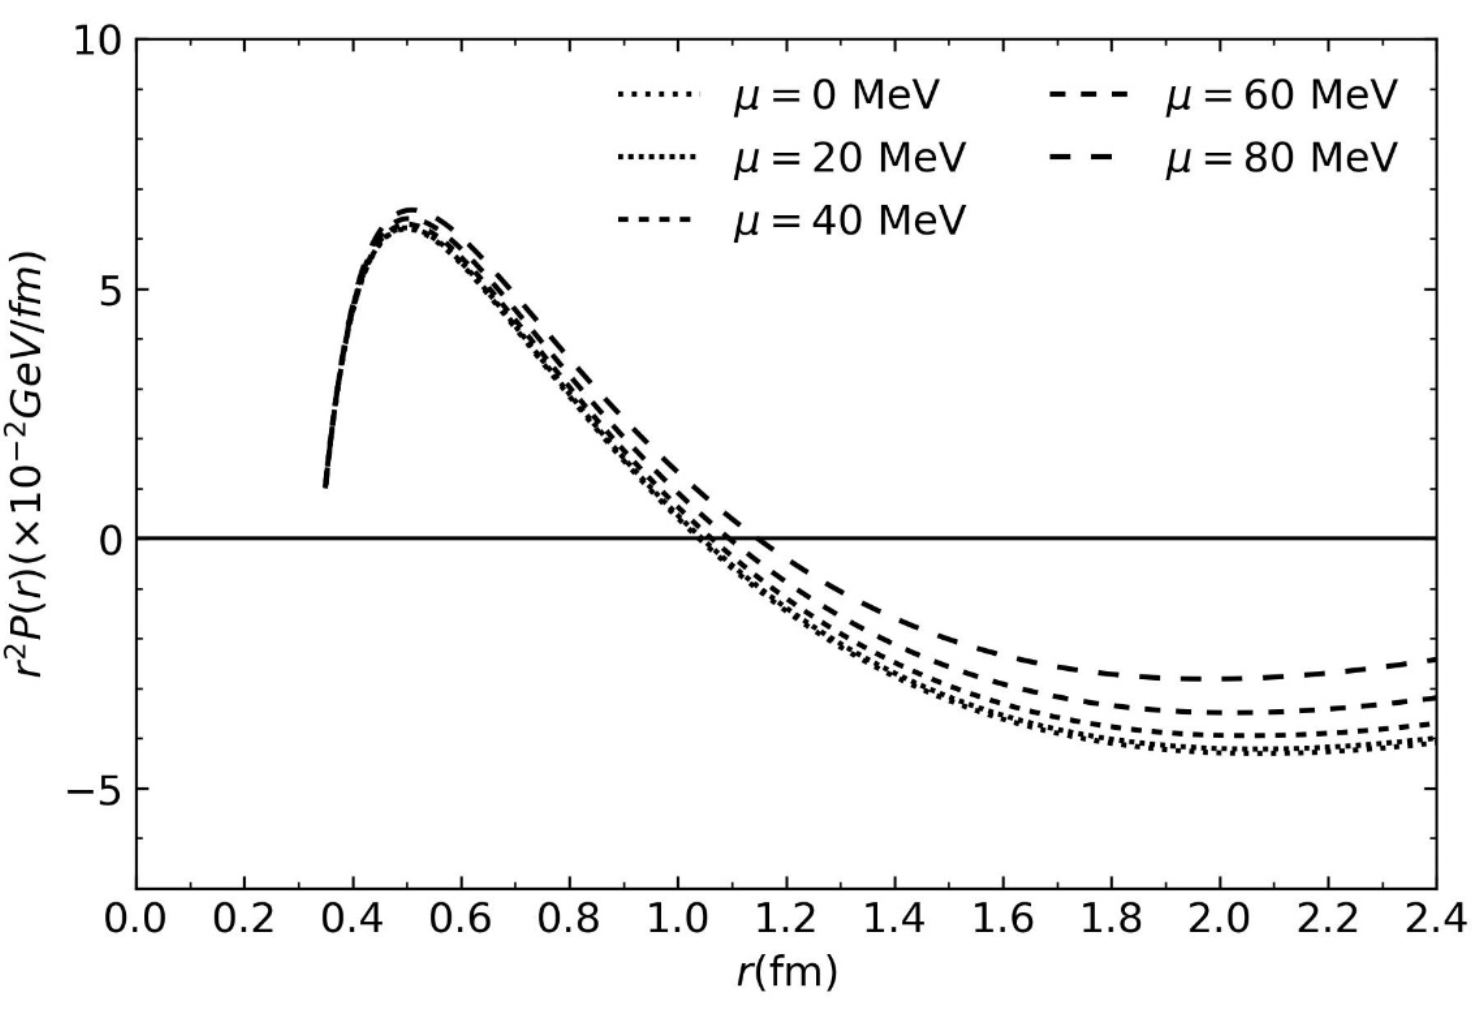
\includegraphics[width=0.58\textwidth]{./Images/TotalPressureTsallis.png}
% \caption[Presión total en el modelo T-MIT bag model]{\emph{Distribución de presión radial en el protón  contra la distancia radial desde el centro para distintos potenciales químicos. El parámetro de Tsallis usado fue $q=1.05$.}}
% \label{fig: Presión total en T-MIT bag model}
% \end{wrapfigure}

% Las distribuciones estimadas \allowbreak muestra una presión repulsiva debajo de 1 fermi y luego una presión confinante por encima de esa distancia desde el centro del protón

% La distribución de presión que resulta de las interacciones de los quarks en el protón contra la distancia radial desde el centro del protón fue obtenida en [referencia de nature]. usando datos experimentales. Una presión repulsiva fuerte cerca del centro del protón se desvanece a una distancia radial de aproximadamente $0.6 \mathrm{\unit{\femto\meter}}$. Más allá de esa distancia, la presión de ligadura aparece. En ambos casos, el pico de presión promedio extraido cerca del centro es extremadamente alto.

% En [26], la distribución de presión de quarks dentro del protón es obtenida considerando un sistema quark aislado sin interacciones de gluones, encontrada usando \gls{gff} usando la expresión para

% \begin{equation}
% {d}_{1}(t) = {d}_{1} (0) \left(1- \frac{t}{{M}^{2}} \right)^{-\alpha}
% \end{equation}

% que viene de la expansión de Gegengabauer del término D (uno de los \gls{gff})

% \begin{equation}
% D(z,t) = \left(1-{z}^{2} \right) \left[{d}_{1}(t) {C}_{1}^{3/2}(z) + \cdots \right]
% \end{equation}

% Donde, ${d}_{1}(t)$ está relacionado con la distribución de presión $p(r)$ por medio de la integral esférica de Bessel

% \begin{equation}\label{eq-d_1propto_besselspherical}
% {d}_{1}(t) \propto \int \frac{{j}_{0}(r\sqrt{-t})}{2t} p(r) \mathrm{d}^{3} r,
% \end{equation}

% donde ${j}_{0}$ es la primera función de Bessel esférica. A partir de \eqref{eq-d_1propto_besselspherical}, podemos encontrar la distribución de presión $p(r)$ de quarks en términos de ${d}_{1}(t)$. La presión está dada por

% \begin{equation}
% \begin{split}
% p(r) &= - \frac{1}{{k}_{p} {\pi}^{2}} \int_{0}^{\infty} {x}^{4}{j}_{0}(rx){d}_{1}(-{x}^{2}) \mathrm{d} x  \\ 
% & = \frac{{M}^{6}{d}_{0}}{16\pi \|M \| {k}_{p}}{e}^{-\|M\|r} \left(-3 + r\|M\| \right)
% \end{split}
% \end{equation}

% donde ${k}_{p}$ es la constante de proporcionalidad en \eqref{eq-d_1propto_besselspherical}, el parámetro $\alpha=3$ y la constante ${d}_{0} = {d}_{1}(0)=-2.04$ están dadas en [nature], mientras que la constante de proporcionalidad ${k}_{p} = 55$ y $\|M\| = 5$ son propuestos para reproducir los resultados de [Nature]

% \begin{wrapfigure}{l}{0.58\textwidth}
% \centering
% 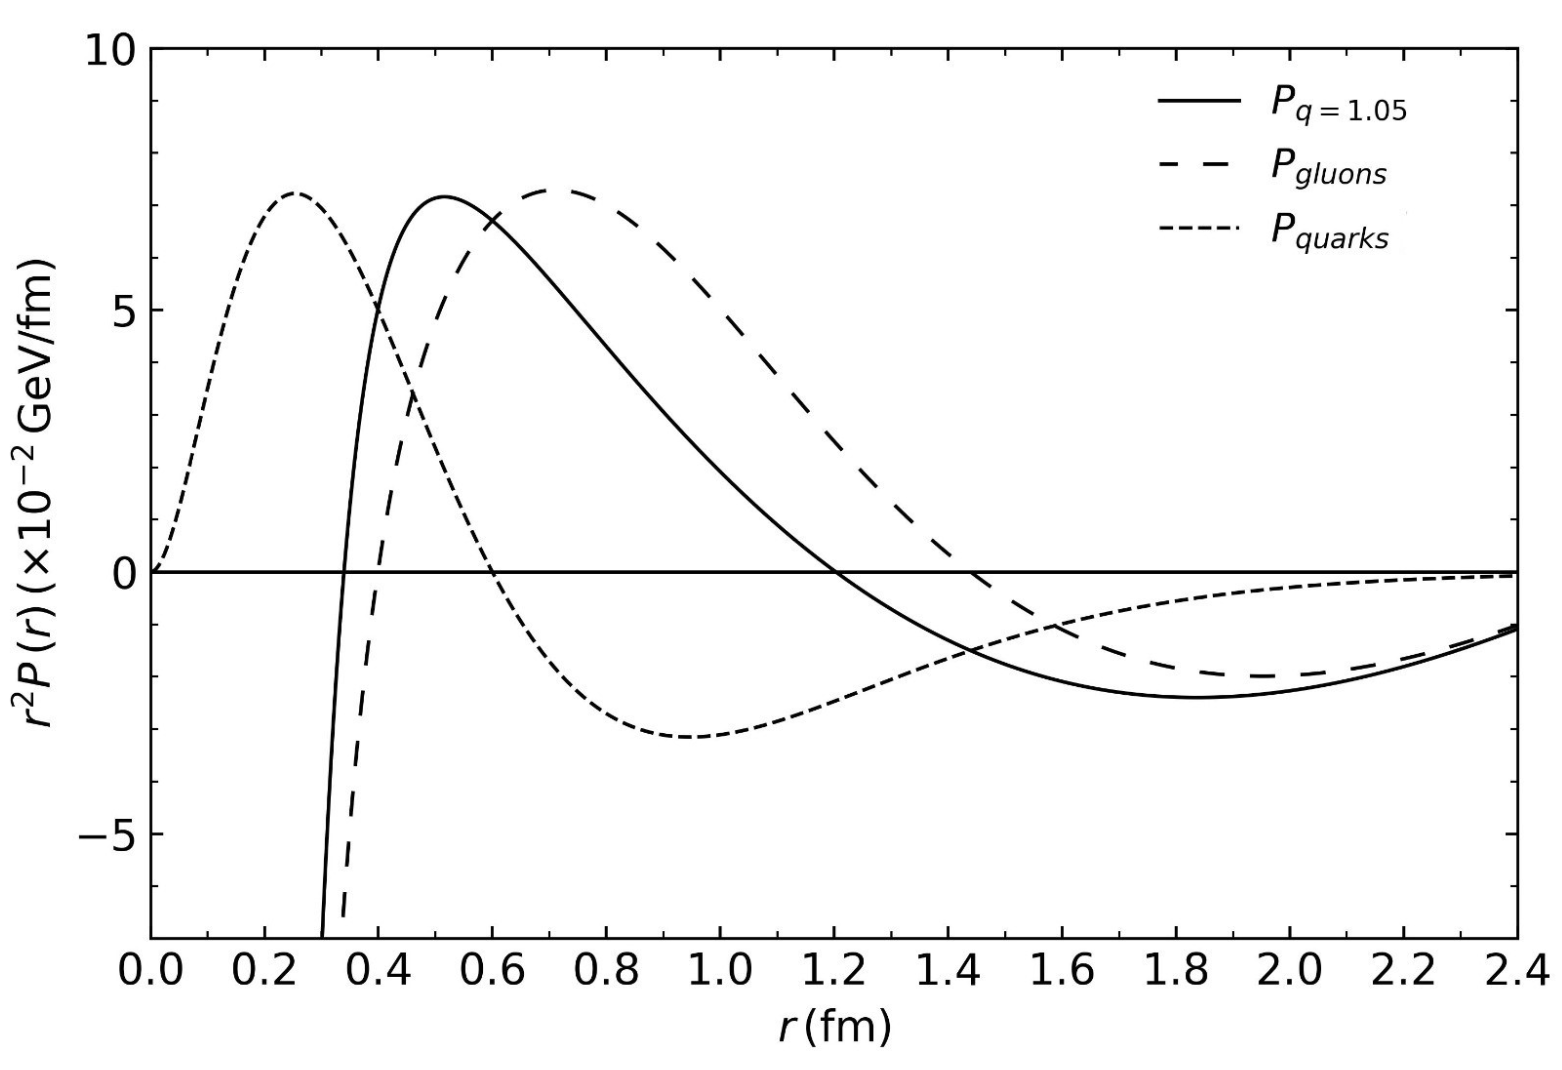
\includegraphics[width=0.58\textwidth]{./Images/PressureDistributionsTot-Q-G.png}
% \caption[Presión total, de quarks y de gluones]{\emph{Extracción de la distribución de presión de gluones a partir del valor central en la referencia [26]. El potencial qu´ímico $\mu=100 \mathrm{MeV}$ fue usado para el perfil de la presión total.}}
% \label{fig: Presión total, de quarks y de gluones}
% \end{wrapfigure}

% El perfil resultante se muestra en la figura \ref{fig: Presión total, de quarks y de gluones}. Usamos esta distribución de presión de quarks para estimar la contribución de los gluones como una substracción del total mostrado arriba. 

\blankpage